%-------------------------------------------------------------------------------
% FIELD ADVANTAGES
%-------------------------------------------------------------------------------
\subsection{Field advantages}
\begin{frame}{Application: game modeling}{Field advantages}

\begin{figure}[ht]
\begin{minipage}[t]{0.5\linewidth}
\vspace{0pt}
Strategic game play:
\begin{itemize}
\item a good test of cognition,
\item easy performance evaluation,
\item a well documented problem.
\end{itemize}
\end{minipage}
\hfill
\begin{minipage}[t]{0.4\linewidth}
\vspace{0pt}
\centering
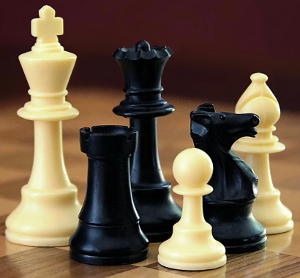
\includegraphics[width=\textwidth]{img/application/chess.png}
\end{minipage}
\end{figure}

\end{frame}

%-------------------------------------------------------------------------------
% CHOSEN GAME: "REVERSI"
%-------------------------------------------------------------------------------
\subsection{Chosen game: ``Reversi"}
\begin{frame}{Application: game modeling}{Chosen game: ``Reversi"}

The game takes place on a 8 by 8 grid: players take turns placing pieces of 
their colour in such a way that at least one line of their opponents pieces are
surrounded. Surrounded pieces change colour, the goal being to have the most 
pieces of one's own colour on the board when the game end.

NB - we can see that pieces on the corners and edges will form configurations of 
interest...

\end{frame}

%-------------------------------------------------------------------------------
% VON NEUMANN'S THEOREM
%-------------------------------------------------------------------------------
\subsection{Von Neumann's theorem}
\begin{frame}{Application: game modeling}{Von Neumann's theorem}

Minimax algorithm is theoretically optimal if applied in an exact manner.

\end{frame}

%-------------------------------------------------------------------------------
% DRAWBACKS OF MINIMAX
%-------------------------------------------------------------------------------
\subsection{Drawbacks of Minimax}
\begin{frame}{Application: game modeling}{Drawbacks of Minimax}

Minimax is exponential so cannot the used in an exact manner. Search depth must 
be capped and heuristics used. A heuristic is the condensation of an expert's 
knowledge: difficult to codify as based on multum in parvo (many tiny factors).

\end{frame}

%-------------------------------------------------------------------------------
% AN ALTERNATIVE
%-------------------------------------------------------------------------------
\subsection{An alternative}
\begin{frame}{Application: game modeling}{An alternative}

Why can have the system develop its own heuristic evaluation through experience?

\end{frame}